\chapter{Модель общей циркуляции океана INMOM}\label{ch:inmsom/ch1}

\section{Математическая постановка задачи}\label{sec:inmsom/ch1/sec1}

\subsection{Базовые уравнения гидротермодинамики океана}
    Систему уравнений крупномасштабной динамики океана в приближениях гидростатики и Буссинеска для сферического слоя на Земле в предположении ее постоянного радиуса можно записать в векторной форме Громеки-Лэмба следующим образом:
		
	\begin{equation} \label{eq:inmsom/1} 
	\begin{array}{c} 
	\displaystyle{\frac{\partial \textbf{U}_h }{\partial t_{} } +\left[\mbox{rot}\textbf{U}\times \textbf{U}\right]_{h} +2 \mathbf{ \Omega } \times \textbf{k}+ \mbox{grad}_{h} \left(\frac{\textbf{U}^{2} }{2^{} } + \frac{p_{} }{\rho _{0} } \right)=F_{h} (\textbf{U})} \\ 
	
	\displaystyle{\frac{\partial \theta }{\partial t} +\textbf{U}\cdot \mbox{grad}\theta =F(\theta )-\frac{\partial R}{\partial z} } \\ 
	
	\displaystyle{\frac{\partial S}{\partial t} + \textbf{U}\cdot \mbox{grad}S=F(S)} \\ 
	
	\displaystyle{\frac{\partial p}{\partial z} =\rho g} \\ 
	
	\displaystyle{\mbox{div} \textbf{U}=0} \\ 
	
	\displaystyle{\rho =\rho (\theta ,S,p)} 
	\end{array} 
	\end{equation} 
	
	Здесь $\textbf{U} = (u, v, w)$ - трехмерный вектор скорости, $[\cdot]_h$ - оператор проекции трехмерного вектора на
	горизонтальную плоскость, $p$ - давление, $\rho_0$ - фоновая плотность (константа по пространству и времени),
	$\rho$ - истинная плотность, $g$ - среднее ускорение свободного падения,
	$\mathbf{ \Omega} $ - угловая скорость вращения Земли, $\theta$ - потенциальная температура морской воды, $S$ - ее соленость,
	$R$ - поток проникающей радиации, $F(\textbf{U}), F(\theta), F(S)$ - операторы мелкомасштабной физики (диффузии и вязкости), конкретный вид
	которых выбирается в зависимости от обстоятельств, $\textbf{k}$ - базисный вектор, направленный вдоль линии действия силы тяжести.
	
	В обобщенной ортогональной сферической системе координат $(x, y, z)$ с метрическими коэффициентами $(r_x, r_y, r_z)$ (коэффициентами Ламе) и с единичными векторами 
	$\textbf{i}$, $\textbf{j}$, $\textbf{k}$,
	направленными вдоль соответствующих координат, операторы
	дифференциальной геометрии записываются следующим образом:
	$$ \mbox{grad} f = \frac{\textbf{i}}{r_x}\d{f}{x} + \frac{\textbf{j}}{r_y}\d{f}{y} + \frac{\textbf{k}}{r_z}\d{f}{z} $$
	$$ \mbox{div} \textbf{F} = \frac{1}{r_x r_y r_z} \left( \d{}{x}(F_x r_y r_z) + \d{}{y}(F_y r_z r_x) + \d{}{z}(F_z r_x r_y) \right) $$
	$$ \mbox{rot} \textbf{F} = \frac{\textbf{i}}{r_y r_z} \left( \d{}{y}(F_z r_z) - \d{}{z}(F_y r_y) \right) + 
	\frac{\textbf{j}}{r_z r_x} \left( \d{}{z}(F_x r_x) - \d{}{x}(F_z r_z) \right) + $$
	$$ + \frac{\textbf{k}}{r_x r_y} \left( \d{}{x}(F_y r_y) - \d{}{y}(F_x r_x) \right) $$
	где $f$ - некоторая скалярная функция, $\textbf{F} = (F_x, F_y, F_z)$ - векторное поле.
	
	В обобщенной ортогональной сферической системе координат $r_z = 1$, а $r_x$ и $r_y$ могут иметь различный вид. Если положить метрические коэффициенты
	не зависящими от координаты $z$ (приближение тонкого сферического слоя), то уравнения будут иметь вид:
	
	\begin{equation} \label{eq:inmsom/2} 
	\begin{array}{c} 
	\displaystyle{ \frac{du}{dt} -\left(l+\frac{1}{r_{x} r_{y} } \left(v\frac{\partial r_{y} }{\partial x} -u\frac{\partial r_{x} }{\partial y} \right)\right)v = -\frac{1}{\rho _{0} } \frac{1}{r_{x} } \frac{\partial p}{\partial x} +\tilde{F}_{u} } \\
	
	\displaystyle{ \frac{dv}{dt} +\left(l+\frac{1}{r_{x} r_{y} } \left(v\frac{\partial r_{y} }{\partial x} -u\frac{\partial r_{x} }{\partial y} \right)\right)u = -\frac{1}{\rho _{0} } \frac{1}{r_{y} } \frac{\partial p}{\partial y} +\tilde{F}_{v} } \\ 
	
	\displaystyle{\frac{\partial p}{\partial z} =\rho g} \\ 
	
	\displaystyle{\frac{d\theta }{dt} =F(\theta )-\frac{\partial R}{\partial z} } \\ 
	
	\displaystyle{\frac{dS}{dt} =F(S)} \\ 
	
	\displaystyle{\frac{1}{r_{x} r_{y} } \left(\frac{\partial ur_{y} }{\partial x} +\frac{\partial vr_{x} }{\partial y} \right)+\frac{\partial w}{\partial z} =0} \\ 
	
	\displaystyle{\rho =\rho (\theta ,S,p)} 
	\end{array} 
	\end{equation} 
	
	Здесь $\displaystyle{\frac{d}{dt} \equiv \d{}{t} + \frac{u}{r_x} \d{}{x} + \frac{v}{r_y}\d{}{y} + w\d{}{z} }$, $l = 2 \Omega sin(\phi)$ - параметр Кориолиса,
	где $\phi$ - географическая широта.
	
	Более подробно про запись уравнений гидротермодинамики океана в обобщенных координатах можно посмотреть, например, здесь \cite{INMOM}, \cite{SuhovPhD}, \cite{GusevPhD}.
	
\subsection{Запись уравнений в сигма-координатах}
	Введем вертикальную координату $\displaystyle{ \sigma = \frac{z + \zeta(x, y, t)}{H(x, y) + \zeta(x, y, t)} }$, где $x$ и $y$ - обобщенные горизонтальные
	координаты, $z$ - направленная вниз обычная вертикальная координата по глубине,
	с началом на невозмущенной поверхности океана, $H$ - глубина океана в состоянии покоя, $\zeta$ - отклонение уровня океана от невозмущенной
	поверхности. На рис. \ref{fig:sigma_levels} схематически изображено распределение $\sigma$-уровней по глубине. 
	
	\begin{figure}[htb!]
	\center
	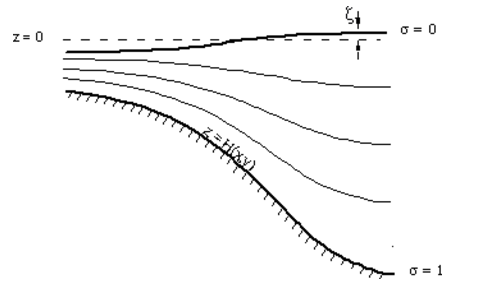
\includegraphics[scale = 0.7]{sigma_plus.png}
	\caption{Схематическое распределение сигма-уровней по глубине}
	\label{fig:sigma_levels}
	\end{figure}
	
	Полагая $h = H + \zeta$ 
	%(эффективная глубина океана)
	и $Z = \sigma h - \zeta$,
	%(геопотенциальная $z$-координата как функция новых координат)
	получим преобразование частных производных при переходе из $z$ в $\sigma$ систему координат:
	$$ \d{}{x} \rightarrow \d{}{x} - \frac{1}{h} \d{Z}{x} \d{}{\sigma} $$
	$$ \d{}{y} \rightarrow \d{}{y} - \frac{1}{h} \d{Z}{y} \d{}{\sigma} $$
	$$ \d{}{z} \rightarrow \frac{1}{h} \d{}{\sigma} $$
	$$ \d{}{t} \rightarrow \d{}{t} - \frac{1}{h}\d{Z}{t}\d{}{\sigma} $$
	
	
	Тогда система (\ref{eq:inmsom/2}) переписывается следующим образом:
	
	\begin{equation} \label{eq:inmsom/3} 
	\begin{array}{c} 
	\displaystyle{\frac{du}{dt} -\left(l+\frac{1}{r_{x} r_{y} } \left(v\frac{\partial r_{y} }{\partial x} -u\frac{\partial r_{x} }{\partial y} \right)\right)v=} \\
	\displaystyle{= -\frac{1}{\rho _{0} } \frac{1}{r_{x} } \left(\frac{\partial p}{\partial x} -\frac{1}{h} \frac{\partial Z}{\partial x} \frac{\partial p}{\partial \sigma } \right)+\tilde{F}_{u} +\frac{1}{h} \frac{\partial }{\partial \sigma } \left(\frac{\kappa }{h} \left(\frac{\partial u}{\partial \sigma } \right)\right)} \\
	
	\displaystyle{\frac{dv}{dt} +\left(l+\frac{1}{r_{x} r_{y} } \left(v\frac{\partial r_{y} }{\partial x} -u\frac{\partial r_{x} }{\partial y} \right)\right)u=} \\
	\displaystyle{= -\frac{1}{\rho _{0} } \frac{1}{r_{y} } \left(\frac{\partial p}{\partial y} -\frac{1}{h} \frac{\partial Z}{\partial y} \frac{\partial p}{\partial \sigma } \right)+\tilde{F}_{v} +\frac{1}{h} \frac{\partial }{\partial \sigma } \left(\frac{\kappa }{h} \left(\frac{\partial v}{\partial \sigma } \right)\right)} \\
	
	\displaystyle{\frac{1}{h} \frac{\partial p}{\partial \sigma } =\rho g} \\
	
	\displaystyle{\frac{d\theta }{dt} = \tilde{F}_{\theta } -\frac{1}{h} \frac{\partial R}{\partial \sigma } } \\
	
	\displaystyle{\frac{dS}{dt} = \tilde{F}_{S} } \\ 
	
	\displaystyle{\frac{\partial h}{\partial t} +\frac{1}{r_{x} r_{y} } \left(\frac{\partial ur_{y} h}{\partial x} +\frac{\partial vr_{x} h}{\partial y} \right)+\frac{\partial \omega }{\partial \sigma } =0} \\
	
	\displaystyle{\rho =\rho (\theta ,S,p)} 
	\end{array}
	\end{equation}
	
	Здесь  $\displaystyle{ \frac{d}{dt} \equiv \d{}{t} + \frac{u}{r_x} \d{}{x} + \frac{v}{r_y}\d{}{y} + \frac{\omega}{h}\d{}{\sigma} }$ и
	$\displaystyle{ \omega = w - \frac{u}{r_x}\d{Z}{x} - \frac{v}{r_y}\d{Z}{y} - \d{Z}{t} }$ - составляющая скорости, нормальная к $\sigma$-поверхности.
	
	Вывод уравнений гидротермодинамики океана при переходе от координаты обычной глубины $z$ к $\sigma$-координате приведен, например,
	в работах \cite{AleskeevZalesny}, \cite{BlumbergMellor}.
	
	\subsection{Граничные условия}

    Система (\ref{eq:inmsom/3}) сопровождается набором граничных и начальных условий.
	На твердых участках границы области ставятся следующие условия: для скорости - непротекание, скольжение на боковой поверхности (равенство нулю компонентов тензора вязких напряжений) и квадратичное трение на дне; для температуры и солености - отсутствие потоков тепла и соли. 
	Рассмотрим условия на свободной поверхности океана $\sigma = 0 $, на которой задаются
	потоки пресной воды, тепла, соли и импульса в следующем виде:

	\bigskip
	- для вертикальной скорости - скорость притока объема воды в бассейн:

	\begin{equation} \label{eq:inmsom/bc1} 
	\displaystyle{ \omega =Q }
	\end{equation} 

	где $Q$ - баланс потока воды на поверхности, задаваемый в единицах скорости.

	\bigskip
	- для импульса:

	\begin{equation} \label{eq:inmsom/bc2} 
	\displaystyle{ \omega \textbf{U}_{h} -\frac{\nu }{h} \frac{\partial \textbf{U}_{h} }{\partial \sigma _{} } =q_{U} } 
	\end{equation} 

	где $q_U$ - поток импульса, нормированный на среднюю плотность воды и состоящий как из напряжения трения ветра на поверхности, так и из импульса, изменяемого в системе за счет изменения объема бассейна.

	\bigskip
	- для температуры и солености:

	\begin{equation} \label{eq:inmsom/bc3} 
	\begin{array}{l} 
	\displaystyle{ {\omega \theta -\frac{\nu _{\theta } }{h_{} } \frac{\partial \theta }{\partial \sigma } =q_{\theta } } } \\ 
	\displaystyle{ {\omega S-\frac{\nu _{S} }{h_{} } \frac{\partial S}{\partial \sigma } =q_{S} } } 
	\end{array} 
	\end{equation} 

	где $q_{\theta}$ и $q_S$ - нормированные потоки тепла и соли, состоящие как из турбулентных потоков, так и из потоков, возникающих в системе за счет изменения объема бассейна.
	
	\bigskip
	- для давления:
	
	\begin{equation} \label{eq:inmsom/bc4} 
	\displaystyle{ p = p_{a} } 
	\end{equation} 
	
	где $p_{a}$ - атмосферное давление на уровне моря.
	
	\subsection{Подготовка к решению системы уравнений гидротермодинамики океана}
	
	\begin{enumerate}
	\item  \textbf{Приведение к дивергентному виду. }
Умножим уравнения для каждой прогностической переменной на $h$. 
Затем прибавим к каждому из них уравнение неразрывности, умноженное на соответствующую переменную.

	\item  \textbf{Симметризация градиента давления.} 
	Представим давление как $p=\tilde{p}+\frac{1}{2} \rho gZ$. 
	Тогда, исключая уравнение гидростатики, с учётом граничных условий получим:

	\begin{equation} \label{eq:inmsom/4}
	\begin{array}{c} 
	\displaystyle{\frac{\partial hu}{\partial t} + T_{u} (u,v,\omega ,h) - h l v = P_{x} -hg\frac{1}{r_x}\frac{\partial \zeta }{\partial x} - \frac{1}{\rho_0 r_x}\frac{\partial p_a}{\partial x} + F_{u} (u,v) + } \\
	\displaystyle{+ \frac{\partial }{\partial \sigma } \left(\frac{\kappa }{h} \left(\frac{\partial u}{\partial \sigma } \right)\right)} \\
	
	\displaystyle{\frac{\partial hv}{\partial t} + T_{v} (u,v,\omega ,h) + h l u = P_{y} -hg\frac{1}{r_y}\frac{\partial \zeta }{\partial y} -\frac{1}{\rho_0 r_y}\frac{\partial p_a}{\partial y} + F_{v} (u,v) + } \\
	\displaystyle{+ \frac{\partial }{\partial \sigma } \left(\frac{\kappa }{h} \left(\frac{\partial v}{\partial \sigma } \right)\right)} \\ 
	
	\displaystyle{\frac{\partial h}{\partial t} +\frac{1}{r_{x} r_{y} } \left(\frac{\partial ur_{y} h}{\partial x} +\frac{\partial vr_{x} h}{\partial y} \right)+\frac{\partial \omega }{\partial \sigma } =0} \\ 
	
	\displaystyle{\frac{\partial \theta }{\partial t} + T_{\theta } (u,v,\omega ,\theta ,h) = F_{\theta } (\theta ) + \frac{\partial }{\partial \sigma } \left(\frac{\kappa _{\theta } }{h} \left(\frac{\partial \theta }{\partial \sigma } \right)\right) - \frac{\partial R}{\partial \sigma } } \\ 
	
	\displaystyle{\frac{\partial S}{\partial t} + T_{S} (u,v,\omega ,S,h) = F_{S} (S) + \frac{\partial }{\partial \sigma } \left(\frac{\kappa _{S} }{h} \left(\frac{\partial S}{\partial \sigma } \right) \right)} \\ 
	
	\displaystyle{\rho =\rho (\theta ,S,p)} 
	\end{array} 
	\end{equation} 
	
	\end{enumerate}

	Здесь введены следующие обозначения:
	
	1. $\kappa$, $\kappa_\theta$, $\kappa_S$ - коэффициенты вертикальной турбулентной вязкости (для $u$ и $v$) и диффузии (для $\theta$ и $S$).

	2. Операторы переноса в (\ref{eq:inmsom/4}) записаны в дивергентной форме
	с добавлением членов, описывающих перенос в криволинейной системе координат:

	\begin{equation} \label{eq:inmsom/5} 
	\begin{array}{c} 
	\displaystyle{T_{u} (u,v,\omega ,h) = \frac{1}{r_x r_y} \left( \frac{\partial hr_{y} uu}{\partial x} + \frac{\partial hr_{x} vu}{\partial y} - h\left(v\frac{\partial r_{y} }{\partial x} - u\frac{\partial r_{x} }{\partial y} \right)v \right) + \frac{\partial \omega u}{\partial \sigma } }\\ 
	
	\displaystyle{T_{v} (u,v,\omega ,h) = \frac{1}{r_x r_y} \left( \frac{\partial hr_{y} uv}{\partial x} + \frac{\partial hr_{x} vv}{\partial y} + h\left(v\frac{\partial r_{y} }{\partial x} - u\frac{\partial r_{x} }{\partial y} \right)u \right) + \frac{\partial \omega v}{\partial \sigma } } \\ 
	
	\displaystyle{T_{\theta } (u,v,\omega ,\theta ,h) = \frac{1}{r_x r_y} \left( \frac{\partial hr_{y} u\theta }{\partial x} + \frac{\partial hr_{x} v\theta }{\partial y} \right) +\frac{\partial \omega \theta }{\partial \sigma } } \\ 
	
	\displaystyle{T_{S} (u,v,\omega ,S,h) = \frac{1}{r_x r_y} \left( \frac{\partial hr_{y} uS}{\partial x} + \frac{\partial hr_{x} vS}{\partial y} \right) +\frac{\partial \omega S}{\partial \sigma } } 
	\end{array} 
	\end{equation} 
	
	С вычислительной точки зрения дивергентная форма обладает полезными свойствами: она автоматически сохраняет первый интеграл переносимой величины при условии непротекания на твердых границах, а квадратичный интеграл 
%	переносимой величины по замкнутой области 
	при условии непротекания на твердых границах и выполнения уравнения неразрывности; она допускает
	простую конечноразностную аппроксимацию.  
	Преимущества дивергентной формы записи уравнений можно посмотреть здесь \cite{ROUCH}.  

	3. Градиенты давления в (\ref{eq:inmsom/4}) записаны в форме:

	\begin{equation} \label{eq:inmsom/6} 
	\begin{array}{c} 
	\displaystyle{P_{x} =-\frac{g h}{2 r_x} \left(\frac{\partial }{\partial x} \int _{0}^{\sigma }h\left(\rho -\sigma \frac{\partial \rho }{\partial \sigma } \right) d\sigma -\sigma \left(\rho \frac{\partial h}{\partial x} -h\frac{\partial \rho }{\partial x} \right)\right)} \\ 
	
	\displaystyle{P_{y} =-\frac{g h}{2 r_y} \left(\frac{\partial }{\partial y} \int _{0}^{\sigma }h\left(\rho -\sigma \frac{\partial \rho }{\partial \sigma } \right) d\sigma -\sigma \left(\rho \frac{\partial h}{\partial y} -h\frac{\partial \rho }{\partial y} \right)\right)} 
	\end{array} 
	\end{equation} 
	
	Одна из трудностей применения сигма-моделей динамики океана связана с наличием погрешности аппроксимации горизонтального градиента давления.
	Из-за погрешности разностной аппроксимации градиентов давления вдоль поверхностей $\sigma = const$ возникают ненулевые скорости и иногда,
	при ярко выраженной стратификации плотности по вертикали и при больших градиентах топографии дна, эти фиктивные скорости могут быть значительными.
	Представление горизонтальных градиентов давления в форме (\ref{eq:inmsom/6}) позволяет уменьшить эти погрешности \cite{INMOM}.

	4. Оператор боковой вязкости в (\ref{eq:inmsom/4}) записывается как дивергенция тензора напряжений:

	\begin{equation} \label{eq:inmsom/7} 
	\begin{array}{c} 
	\displaystyle{F_{u} (u,v)=\frac{1}{r_x r_{y}^2 } \frac{\partial }{\partial x} \left(r_{y} ^{2} KD_{T} h\right)+\frac{1}{r_{x}^2 r_y } \frac{\partial }{\partial y} \left(r_{x} ^{2} KD_{S} h\right)} \\ 
	
	\displaystyle{F_{v} (u,v)=-\frac{1}{r_{x}^2 r_y} \frac{\partial }{\partial y} \left(r_{x} ^{2} KD_{T} h\right)+\frac{1}{r_x r_{y}^2} \frac{\partial }{\partial x} \left(r_{y} ^{2} KD_{S} h\right)} 
	\end{array} 
	\end{equation} 

	Здесь $\textit{K}$ - коэффициент вязкости, а $D_T$ и $D_S$ - компоненты тензоров напряжений сжатия-растяжения и сдвига соответственно:

	\begin{equation} \label{eq:inmsom/8} 
	\begin{array}{c} 
	\displaystyle{D_{T} =\frac{r_{y} }{r_{x} } \frac{\partial }{\partial x} \left(\frac{u}{r_{y} } \right)-\frac{r_{x} }{r_{y} } \frac{\partial }{\partial y} \left(\frac{v}{r_{x} } \right)} \\ 
	
	\displaystyle{D_{S} =\frac{r_{x} }{r_{y} } \frac{\partial }{\partial y} \left(\frac{u}{r_{x} } \right)+\frac{r_{y} }{r_{x} } \frac{\partial }{\partial x} \left(\frac{v}{r_{y} } \right)} 
	\end{array} 
	\end{equation} 

	Операторы диссипации для скоростей написаны в упрощенной форме вдоль сигма-поверхностей \cite{INMOM}, \cite{NCARClimateSystemModel}.

	5. Оператор горизонтального турбулентного обмена для температуры и солености реализован в виде суммы изопикнической диффузии и 
	вихревого переноса Гента-Маквильямса \cite{NCARClimateSystemModel}, \cite{OceanicIsopycnalMixingbyCoordinateRotation} %one more citation should be here, see mag diploma

	\begin{equation} \label{eq:inmsom/9} 
	\begin{array}{c} 
	\displaystyle{D(S)=div(\stackrel{\frown}{K}gradS)} \\ 
	
	\displaystyle{\stackrel{\frown}{K}=\left(\begin{array}{ccc} {\mu } & {0} & {-\mu \alpha _{x} } \\ 
								    {0} & {\mu } & {-\mu \alpha _{y} } \\ 
								    {-\mu \alpha _{x} } & {-\mu \alpha _{y} } & {\mu (\alpha _{x} ^{2} +\alpha _{y} ^{2} )} 
						 \end{array}
		      \right)+\left(\begin{array}{ccc} {0} & {0} & {\gamma \mu \beta _{x} } \\ {0} & {0} & {\gamma \mu \beta _{y} } \\ 
						       {-\gamma \mu \beta _{x} } & {-\gamma \mu \beta _{y} } & {0} 
				    \end{array}\right)} 
	\end{array} 
	\end{equation} 

	где $\mu$ - коэффициент боковой диффузии, $\gamma $ - коэффициент пропорциональности, обычно полагающийся равным 1, 
	$\displaystyle{ \alpha _{x} =\frac{\partial \rho _{pot} /\partial x}{\partial \rho _{pot} /\partial \sigma } }$, 
	$\displaystyle{ \alpha _{y} =\frac{\partial \rho _{pot} /\partial y}{\partial \rho _{pot} /\partial \sigma } }$, 
	$\displaystyle{ \beta _{y} =\alpha _{y} - \frac{Z_{y} }{h} }$.
	$\displaystyle{ \beta _{x} =\alpha _{x} -\frac{Z_{x} }{h} }$.
	Первое слагаемое тензора описывает диффузию вдоль поверхностей постоянной потенциальной плотности, второе - процесс переноса со скоростями:

	\[U_{gm} =\frac{\partial }{\partial z} \left(\gamma \mu \beta _{x} \right),\quad V_{gm} =\frac{\partial }{\partial z} \left(\gamma \mu \beta _{y} \right),\quad W_{gm} =div_{h} \left(\gamma \mu \beta _{x} ,\gamma \mu \beta _{y} \right).\] 
		
	
\section{Численная реализация модели}\label{sec:inmsom/ch1/sec2}
\subsection{Пространственная аппроксимация}
	В модели используется сетка 'C' по классификации Аракавы \cite{ARAKAWA1977}, \cite{ARAKAWA1976}
	в общем случае нерегулярная по долготе и широте и неравномерная по вертикали.
	Разобьем область $x \in [x_0, x_{max}], \quad y \in [y_0, y_{max}] $, куда входит область, на которой рассматривается система уравнений (\ref{eq:inmsom/4}),
	на элементарные ячейки, которые будут иметь форму прямоугольников:
	
	$$ \{ (x, y, \sigma) : x_{m-1} < x < x_{m}, \quad y_{n-1} < y < y_{n}, \quad \sigma_{k-1} < \sigma < \sigma_{k} \} $$
	
	Для решения системы уравнений (\ref{eq:inmsom/4}) применяется техника построения разностных аппроксимаций по пространству второго порядка точности на разнесенной 
	'C'-сетке. На рис. \ref{fig:3dgrid} показаны распределения переменных в каждой сеточной ячейке. 
	
	\begin{figure}[htb!]
	\center
	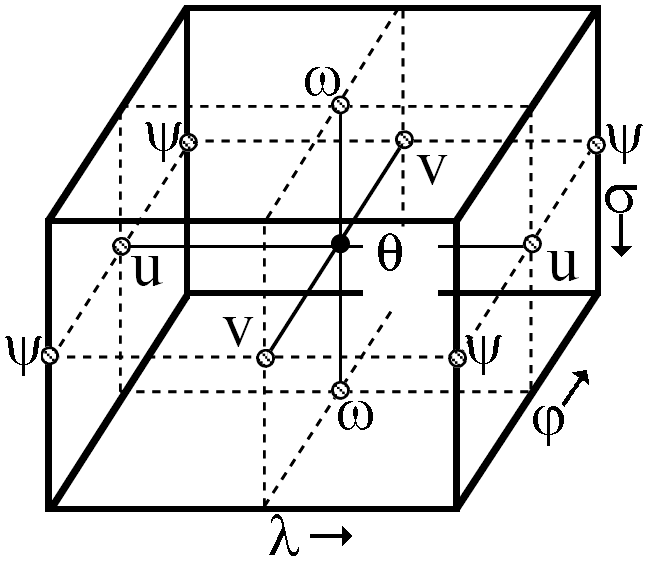
\includegraphics[scale = 0.3]{grid.png}
	\caption{Распределение переменных на ячейке модельной сетки}
	\label{fig:3dgrid}
	\end{figure}
	
	Внутри ячейки располагаются
	скалярные величины $(\theta, S, p, \rho, \zeta)$. В этих же точках задана топография дна и рассчитывается дивергенция скорости. На соответствующих гранях
	распределяются потоковые переменные, такие как компоненты вектора скорости $(u, v, \omega)$, а также производные скалярных величин по соответствующим
	направлениям. При этом скорости расположены точно в центре отрезка, соединяющего две соседние точки скалярных величин, что необходимо для получения
	правильной конечноразностной аппроксимации по пространству \cite{ROUCH}, \cite{MARCHUK}. Относительная завихренность определяется в центрах вертикальных ребер ячеек, там же
	определяется параметр Кориолиса $l$.
	
	При построении разностных схем особое место уделяется тому, чтобы сохранялись свойства симметрии разностных 
	аналогов операторов, которые выполняются для дифференциальной задачи. Это позволяет автоматически удовлетворять энергетическим соотношениям
	в разностной задаче, справедливым для дифференциальной. Методика построения пространственных разностных аппроксимаций хорошо изложена, например, здесь \cite{ROUCH}, \cite{MARCHUK}.
	
\subsection{Схема по времени}
	В модели используется двухслойная схема по времени. На начало шага интегрирования $n+1$ считаются известными все величины на шаге $n$. 
	Для построения согласованной схемы решения используется линеаризация нелинейных слагаемых. 
	Это означает, что некоторые переменные, входящие в состав таких слагаемых, считаются неизменными на протяжении шага интегрирования по времени. 
	В частности, после интегрирования на предыдущем шаге по времени на текущий момент имеются скорости течений $u^n$, $v^n$, уровень моря $\zeta^n$, полная толщина океана $h^n$. 
	После расчёта потоков объёма, тепла, соли и импульса для текущего шага по времени можно с помощью уравнения неразрывности рассчитать новую толщину океана $h^{n+1}$ и вертикальную скорость.
	На этом уравнении неразрывности, которое считается фиксированным, и основаны процессы переноса всех субстанций на новом шаге по времени. 
	Аналогично, линеаризации подвергается потенциальная плотность. 
	Эти величины, в свою очередь позволяют рассчитать коэффициенты турбулентных диффузии и вязкости, 
	углы наклона нейтральных поверхностей и построить линеаризованные операторы бокового и вертикального турбулентного обменов. 
	Для операторов переноса используется дополнительный этап предиктора, а в окончательный оператор входит линейная комбинация решения с явного шага и решения с шага предиктор. 
	В операторах диффузии и вязкости по горизонтали переменные берутся без коррекции с явного шага, а по вертикали – с неявного. 
	Для скорости задача расщепляется на два основных этапа: перенос-диффузия и адаптация к полю давления.
	Ниже приводится подробное описание интегрирования модели на одном шаге по времени.
	
\section{Общая схема решения системы уравнений гидротермодинамики океана}\label{sec:inmsom/ch1/sec3}
Алгоритм численного решения системы уравнений (\ref{eq:inmsom/4}) основан на методе расщепления Г.И. Марчука \cite{MARCHUK}. Используется только расщепление по физическим процессам. 
Схему работы сигма-модели INMOM можно описать следующим образом: инициализация, основной цикл по времени, финализация. Основной цикл по времени состоит из следующих этапов:

\begin{enumerate}
\item  Определение текущего модельного времени (подпрограмма model\_time\_def):

\begin{equation} \label{eq:inmsom/10} 
  \displaystyle{ t = t(\tau ,n)   }
\end{equation} 

где $t$ - текущее время, $n$ - номер шага, $\tau $ - величина основного шага по времени в секундах. 

\item  Задание потоков для прогностических переменных на поверхности и открытых границах ('жидких'), соответствующих текущему моменту времени:

\begin{equation} \label{eq:inmsom/11} 
   \displaystyle{ f_{bound} =f_{bound} (t) }
\end{equation} 

где в качестве $f_{bound} $ выступают температура, соленость и данные на свободной поверхности океана и 'жидких' границах 
(для данных на океанической сетке подпрограмма oc\_data\_time\_interpol) и 
характеристики атмосферы (для данных на атмосферной сетке интерполяция по времени - подпрограмма atm\_data\_time\_interpol, 
и интерполяция по пространству - подпрограмма atm\_data\_spatial\_interpol).

\item Расчёт компонентов тензора горизонтальных напряжений для полных трёхмерных скоростей и средних по глубине (подпрограмма stress\_components).

\begin{equation} \label{eq:inmsom/12} 
\begin{array}{l} 
\displaystyle{ D_{T} =\frac{r_{y} }{r_{x} } \frac{\partial }{\partial x} \left(\frac{u^{n} }{r_{y} } \right)-\frac{r_{x} }{r_{y} } \frac{\partial }{\partial y} \left(\frac{v^{n} }{r_{x} } \right) } \\ 

\displaystyle{ D_{S} =\frac{r_{x} }{r_{y} } \frac{\partial }{\partial y} \left(\frac{u^{n} }{r_{x} } \right)+\frac{r_{y} }{r_{x} } \frac{\partial }{\partial x} \left(\frac{v^{n} }{r_{y} } \right) }
\end{array} 
\end{equation} 

\item Расчёт коэффициентов горизонтального турбулентного обмена по Смагоринскому, при этом от вязкости рассчитывается и среднее по глубине:

\begin{equation} \label{eq:inmsom/13} 
\displaystyle{ \mu =\mu _{ref} +smag(D_{T}^{2} +D_{S}^{2} ) } 
\end{equation} 

где $\mu_{ref}$ - фоновое значение коэффициента, $smag$ - функция от модуля тензора напряжений (подпрограмма smagorinsky\_coeff).

\item  Расчет углов наклона для универсальной диффузии (подпрограмма diffusion\_slopes).

\item  Расчет потоков на поверхности (подпрограмма sea\_surface\_fluxes) и дне (подпрограмма sea\_bottom\_fluxes).

\item Расчёт новых толщины океана и вертикальной скорости (подпрограмма hhq\_vertical\_velocity), согласованных с уравнением неразрывности:

\begin{equation} \label{eq:inmsom/14} 
\begin{array}{l} 
\displaystyle{ h^{n+1} = h^n + \tau \left( Q^n - \frac{1}{r_x r_y}(\d{\overline{u}^n r_y h^n}{x} + \d{\overline{v}^n r_x h^n}{y}) \right) } \\
 
\displaystyle{ \omega^n = \int_1^\sigma \left( \frac{1}{r_x r_y}(\d{u'^n r_y h^n}{x} + \d{v'^n r_x h^n}{y}) + Q^n \right) d\sigma  }
\end{array} 
\end{equation} 

где $Q^n$ – поток объёма на поверхности на текущий момент времени, 
$u'^n = u^n - \overline{u}^n$, $v'^n = v^n - \overline{v}^n$,
$\overline{u}^n = \int_0^1 u^n d \sigma$, $\overline{v}^n = \int_0^1 v^n d \sigma$
 
\item Расчёт коэффициентов вертикального обмена. Используется один из вариантов:
	а) Параметризация PP (Pacanowski-Philander) \cite{ParameterizationofVerticalMixing}:
	
	\begin{equation} \label{eq:inmsom/15}
	  \displaystyle { Ri = Ri(\rho _{pot} ^{n} ,u^{n} ,v^{n} ),\quad \nu = \nu(Ri) }
	\end{equation}
	где $Ri$ - число Ричардсона, $\nu $ - коэффициент вертикальной диссипации, который 	свой для скорости, температуры и солености 
	(подпрограммы richnum и ppmix).
	
%	б) Параметризация Монина-Обухова.
	
	б) Параметризация Меллора-Ямады (подпрограммы Mellor\_Yamada\_gendis и turb\_tran\_diff) \cite{MellorYamada}.

\item Расчёт температуры и солёности (подпрограмма tracer\_tran\_diff):

а) Шаг предиктор. Используется градиентная форма записи при фиксированной по времени глубине и только для оператора переноса:

\begin{equation} \label{eq:inmsom/16} 
\begin{array}{l} 
\displaystyle{ \frac{\theta^{pred}_{i,j,k} - \theta^n_{i,j,k}}{\tau} + } \\
\displaystyle{ + \frac{1}{2 (\Delta x \Delta y h^n)_{i,j}} ( (u^n h^n \Delta y)_{i+1/2,j,k} (\theta^n_{i+1,j,k} - \theta^n_{i,j,k}) + } \\
\displaystyle{+ (u^n h^n \Delta y)_{i-1/2,j,k} (\theta^n_{i,j,k} - \theta^n_{i-1,j,k}) ) + } \\
\displaystyle{ + \frac{1}{2 (\Delta x \Delta y h^n)_{i,j}} ( (v^n h^n \Delta x)_{i,j+1/2,k} (\theta^n_{i,j+1,k} - \theta^n_{i,j,k}) + } \\
\displaystyle{+ (v^n h^n \Delta x)_{i,j-1/2,k} (\theta^n_{i,j,k} - \theta^n_{i,j-1,k}) ) + } \\
\displaystyle{ + \frac{1}{2 h^n_{i,j}} \left( \omega^n_{i,j,k+1/2}(\theta^n_{i,j,k+1} - \theta^n_{i,j,k}) + \omega^n_{i,j,k-1/2}(\theta^n_{i,j,k} - \theta^n_{i,j,k-1}) \right) = 0 }
\end{array} 
\end{equation} 

б) Шаг корректор. Используется дивергентная форма записи и полное уравнение, значения с шага предиктор используются только в операторе переноса:
\begin{equation} \label{eq:inmsom/17} 
\begin{array}{l} 
\displaystyle{ \frac{h^{n+1} \theta^{n+1}_{i,j,k} - h^n \theta^n_{i,j,k}}{\tau} + } \\
\displaystyle{ + \frac{1}{2 (\Delta x \Delta y)_{i,j}} ( (u^n h^n \Delta y)_{i+1/2,j,k} (\theta^{corr}_{i+1,j,k} - \theta^{corr}_{i,j,k}) + } \\
\displaystyle{+ (u^n h^n \Delta y)_{i-1/2,j,k} (\theta^{corr}_{i,j,k} - \theta^{corr}_{i-1,j,k}) ) + } \\
\displaystyle{ + \frac{1}{2 (\Delta x \Delta y)_{i,j}} ( (v^n h^n \Delta x)_{i,j+1/2,k} (\theta^{corr}_{i,j+1,k} - \theta^{corr}_{i,j,k}) + } \\
\displaystyle{+ (v^n h^n \Delta x)_{i,j-1/2,k} (\theta^{corr}_{i,j,k} - \theta^{corr}_{i,j-1,k}) ) + } \\
\displaystyle{ + \frac{1}{2 h^n_{i,j}} ( \omega^n_{i,j,k+1/2}(\theta^{corr}_{i,j,k+1} - \theta^{corr}_{i,j,k}) + \omega^n_{i,j,k-1/2}(\theta^{corr}_{i,j,k} - \theta^{corr}_{i,j,k-1}) ) = } \\
\displaystyle{ = D(\mu, \nu, \alpha_x, \alpha_y, \theta^n, \theta^{n+1}) - \d{R}{\sigma}}
\end{array} 
\end{equation} 

Здесь $\theta$ - потенциальная температура в заданном узле и моменте времени, 
%$T$ - оператор переноса скаляра как функция скоростей, скаляра и глубины, 
$D$ - совокупность операторов боковой и вертикальной диффузии как функция коэффициентов, углов наклона изонейтральных поверхностей и искомого скаляра, 
$R$ - вертикальный поток проникающей радиации. 
В операторах переноса: $\theta^{corr} = \alpha \theta^{pred} + (1 - \alpha) \theta^n$, где в случае $\alpha = 0$ получается явная схема Эйлера, 
являющаяся для кососимметричных операторов безусловно неустойчивой с коэффициентом перехода $T = \sqrt{1 + C^2}$, где $C$ - число Куранта; 
в случае $\alpha = 1$ получается схема Мацуно с коэффициентом перехода $T = \sqrt{(1 - C^2)^2 + C^2}$, являющаяся условно устойчивой и обладающая численной диффузией \cite{ROUCH}. 
В случае $\alpha = 0.5$ получается схема Хойна с коэффициентом перехода $T = \sqrt{1 + \frac{C^4}{4}}$, являющаяся безусловно неустойчивой, но с более слабой степенью расходимости, нежели схема Эйлера \cite{ROUCH}.

Аналогичное получается уравнение для солёности, за исключением источника радиации. 

\item Расчёт переноса и диффузии для компонентов скорости (подпрограмма uv\_tran\_diff). 

Делается аналогично процедуре для температуры и солёности с той разницей, 
что в адвективные слагаемые добавляются метрические члены, связанные с кривизной системы координат, и оператор вязкости задаётся через тензор вязких напряжений. 
При необходимости используется оператор бигармонической вязкости, который получается двукратным применением оператора гармонической.

\item Расчёт плотностей $\rho^{n+1}$ и $\rho_{pot}^{n+1}$ по обновлённым значениям температуры и солёности. 

Использование обновлённых значений вместо предыдущих позволяет повысить устойчивость алгоритма по скорости внутренних волн, который является условно устойчивым.

\item Расчёт изменения трёхмерной скорости за счёт градиентов давления, вызванного неоднородностью поля плотности (подпрограмма pressure\_gradients): 

\begin{equation} \label{eq:inmsom/18} 
\begin{array}{l} 
\displaystyle{ \d{u}{t} = P_x = } \\
\displaystyle{= -\frac{g}{2}r_y \left( \d{}{x} \int_0^\sigma h^{n+1} (\rho^{n+1} - \sigma \d{\rho^{n+1}}{\sigma}) d\sigma - \sigma (\rho^{n+1}\d{h^{n+1}}{x} - h^{n+1}\d{\rho^{n+1}}{x}) \right) } \\
\displaystyle{ \d{v}{t} = P_y = } \\
\displaystyle{= -\frac{g}{2}r_x \left( \d{}{y} \int_0^\sigma h^{n+1} (\rho^{n+1} - \sigma \d{\rho^{n+1}}{\sigma}) d\sigma - \sigma (\rho^{n+1}\d{h^{n+1}}{y} - h^{n+1}\d{\rho^{n+1}}{y}) \right) }
\end{array} 
\end{equation} 

\item Расчёт правых частей для двумерных скоростей, обусловленных градиентом атмосферного давления.

\item Разделение скоростей на бароклинные и баротропных составляющие (подпрограмма depth\_ave): $u' = u - \overline{u}$, $v' = v - \overline{v}$, $\overline{u} = \int_0^1 u d\sigma$, $\overline{v} = \int_0^1 v d\sigma$.

\item Бароклинная адаптация:

\begin{equation} \label{eq:inmsom/19} 
\begin{array}{l} 
\displaystyle{ \frac{u'^{n+1}}{\tau} - l v'^{n+1} = f_u } \\
\displaystyle{ \frac{v'^{n+1}}{\tau} + l u'^{n+1} = f_v }
\end{array} 
\end{equation} 
где в правой части располагаются слагаемые с предыдущего шага. 
%Ввиду разнесённых сеток для скоростей строится энергетически согласованная пространственная аппроксимация.

\item Баротропная адаптация:

В силу высокой скорости внешних гравитационных волн задачу для них целесообразно реализовать неявным методом. 
Задачу удобно сформулировать в виде полных потоков $U$ и $V$, равных произведению скорости на глубину. 
После вынесения всех источников (атмосферного давления) и слагаемых с предыдущего шага в правую часть мы приходим к системе уравнений (система уравнений мелкой воды):

\begin{equation} \label{eq:inmsom/20} 
\begin{array}{l} 
\displaystyle{ \frac{U^{n+1}}{\tau} - l V^{n+1} + gh\frac{1}{r_x}\d{\zeta^{n+1}}{x} = f_u} \\
\displaystyle{ \frac{V^{n+1}}{\tau} + l U^{n+1} + gh\frac{1}{r_y}\d{\zeta^{n+1}}{y} = f_v} \\
\displaystyle{ \frac{\zeta^{n+1}}{\tau} + \frac{1}{r_x r_y} \left( \d{r_y U^{n+1}}{x} + \d{r_x V^{n+1}}{y} \right) = f_\zeta}
\end{array} 
\end{equation} 

Необходимо использование инструмента для решения систем линейных алгебраических уравнений. При этом желательно матрицу системы рассчитывать один раз в самом начале расчёта. Этого можно добиться, представив глубину в слагаемых при градиентах уровня как сумму невозмущённой глубины и уровня моря, а затем перенеся слагаемые с уровнем в правую часть.

\end{enumerate}

На этом шаг по времени задачи динамики океана заканчивается. Цикл повторяется до достижения нужного момента расчётного времени

\section{Система оперативного моделирования Северного Ледовитого океана и прилегающих к нему акваторий}\label{sec:inmsom/ch1/sec4}

Для воспроизведения текущего состояния и краткосрочного прогноза гидротермодинамики Северного Ледовитого океана и прилегающих к нему акваторий на основе вышеописанной сигма-модели общей циркуляции океана INMOM была подготовлена ее региональная версия INMOM-Арктика с пространственным разрешением $\sim$ 3,7 км \cite{ChaplyginINMOM2021}.

На открытых границах модельной области используются данные по температуре, солености,
горизонтальной скорости и уровню моря из модели более обширной области. Эти данные берутся из базы данных продукта CMEMS. Для учета приливного воздействия в модели INMOM-Арктика на открытых границах задается временной ход приливного уровня моря из данных атласа TPXO 9. 

Для расчета атмосферного воздействия используются данные глобального реанализа атмосферной циркуляции ERA5 с пространственным разрешением 0,25×0,25° с дискретностью по времени 1 ч. 

Оценки точности восстановления полей температуры и солености по модели INMOM-Арктика на сезонном масштабе проводились по данным буев-профилографов ARGO в ретроспективных расчетах циркуляции Северного Ледовитого океана за период с 1 марта по 31 августа 2020 г. без усвоения данных наблюдений.
На рис. \ref{fig:INMOM-DARTs} представлены вертикальные профили температуры и солености в Норвежском море по данным буев-профилографов ARGO №6903557 и 3901619 в точках их всплытия с координатами 2,9146°W, 71,0783°N и 4,966°W, 63,242°N соответственно. Модель INMOM-Арктика адекватно воспроизводит вертикальную структуру вод в этих точках: воспроизводятся точки перегиба на вертикальных профилях и глубины верхнего перемешанного слоя с погрешностью в несколько метров.

\begin{figure}[htb!]
	\center
	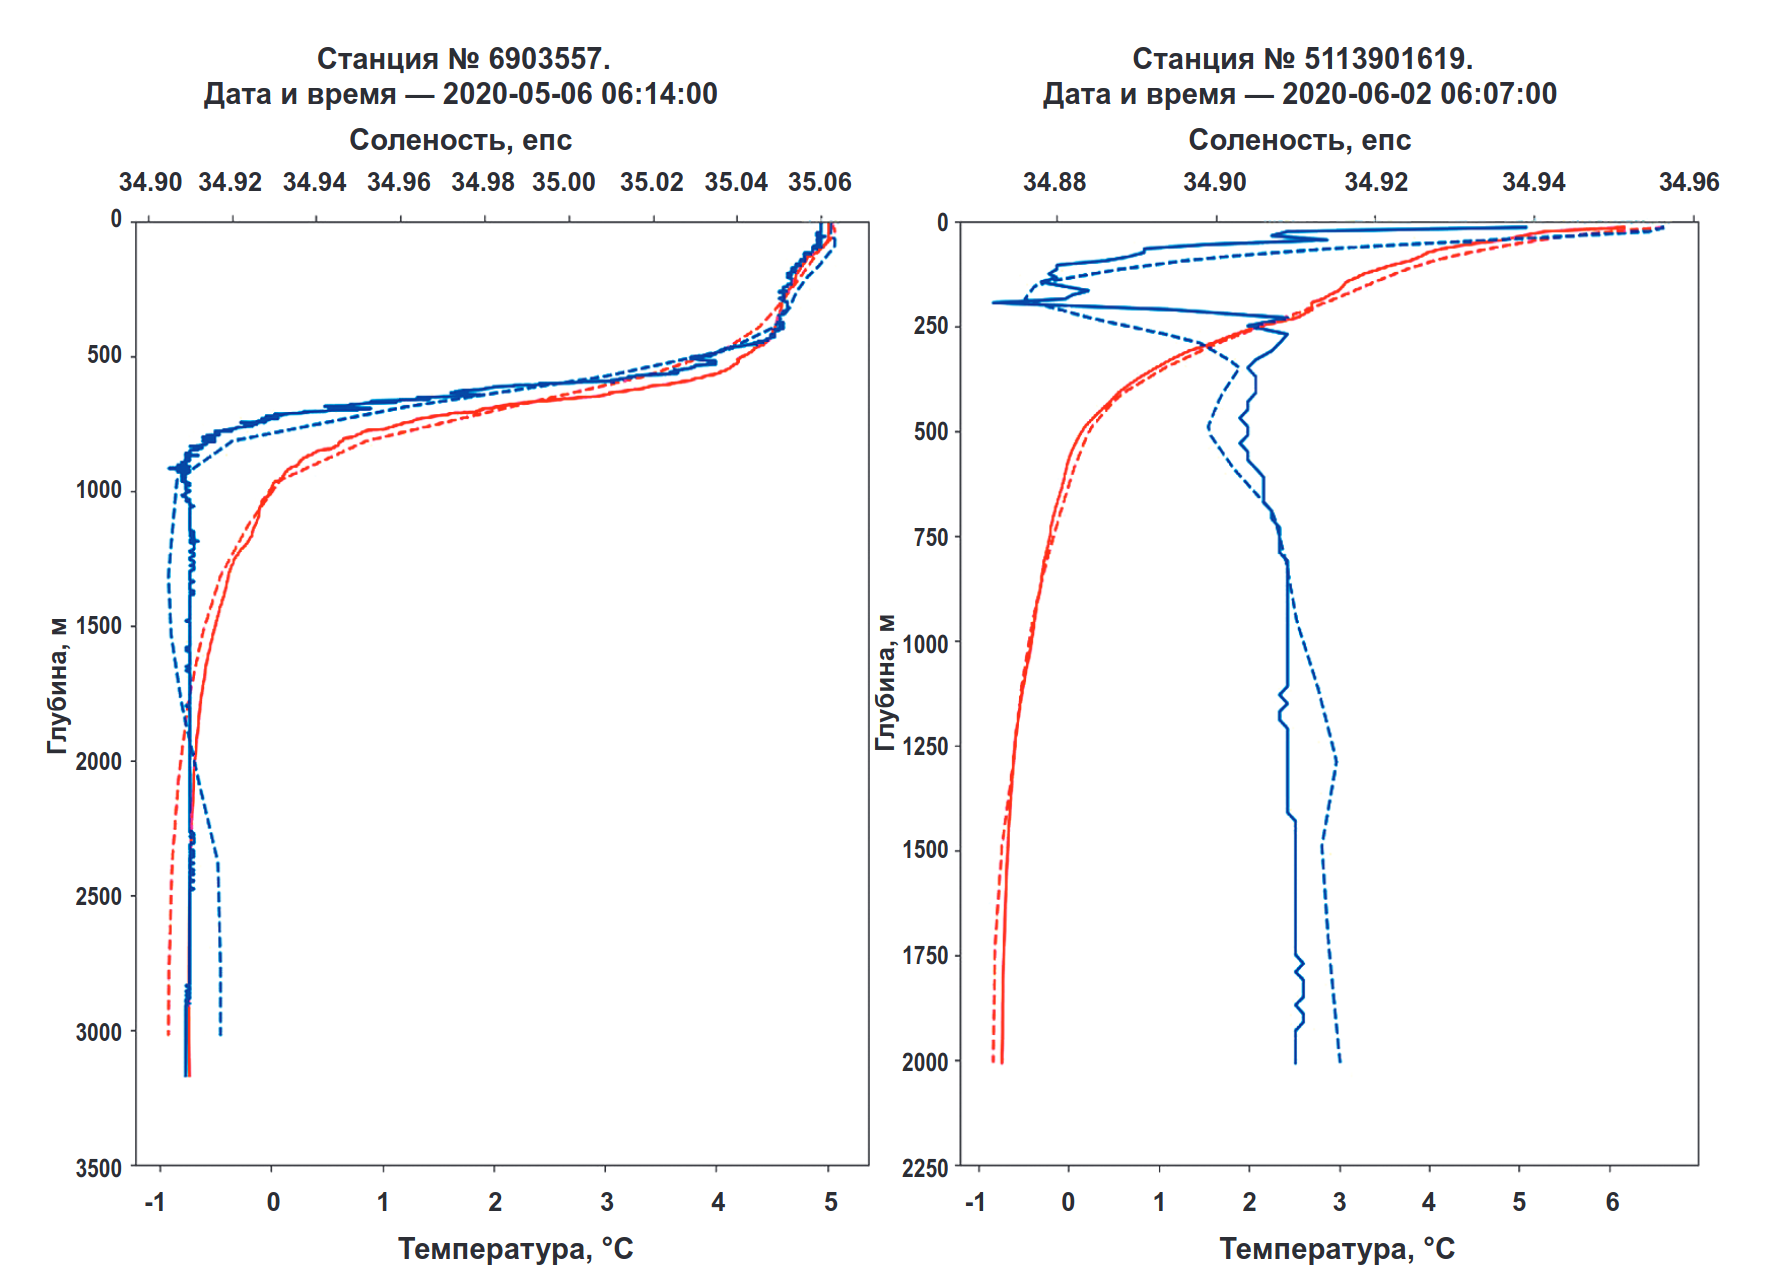
\includegraphics[scale = 0.3]{INMOM-DARTs.png}
	\caption{Рассчитанные (прерывистые красная и синяя кривые соответственно) и измеренные (сплошные красная и синяя кривые соответственно) профили температуры и солености для станций № 6903557 (2,9146°W, 71,0783°N) (а) и № 3901619 (4,966°W, 63,242°N) (б)}
	\label{fig:INMOM-DARTs}
\end{figure}

Результаты сравнения расчетов и данных наблюдений свидетельствуют, что модель INMOM-Арктика с использованием предложенных условий на открытых границах позволяет корректно воспроизводить циркуляцию Северного Ледовитого океана.

\FloatBarrier